\documentclass[12pt,a4paper]{article}

% ============================
% PAQUETES ESENCIALES
% ============================
\usepackage[spanish]{babel}        % Idioma español
\usepackage[utf8]{inputenc}        % Codificación de caracteres
\usepackage[T1]{fontenc}           % Codificación de fuentes

% Configuración de página según APA 7ma edición
\usepackage[top=2.54cm, bottom=2.54cm, left=2.54cm, right=2.54cm]{geometry}
\usepackage{setspace}              % Para interlineado doble
\doublespacing                     % Interlineado doble en todo el documento

% Fuentes Times New Roman
\usepackage{mathptmx}              % Fuente Times New Roman y matemáticas

% Paquetes para matemáticas
\usepackage{amsmath,amssymb,amsthm}

% Para insertar imágenes
\usepackage{graphicx}
\graphicspath{ {./images/} }       % Ruta a la carpeta de imágenes

% Formato APA
\usepackage{apacite}               % Para citas y referencias APA
\usepackage{fancyhdr}              % Para encabezados y pies de página

% Configuración de encabezados y pies de página
\pagestyle{fancy}
\fancyhf{}
\fancyhead[R]{\thepage}            % Número de página en esquina superior derecha
\renewcommand{\headrulewidth}{0pt} % Sin línea de encabezado

% ============================
% PORTADA SEGÚN NORMA APA
% ============================
\begin{document}
\begin{titlepage}
    \centering
    \vspace*{2cm}
    
    {\LARGE \textbf{Ecuaciones Diferenciales Homogéneas y Coeficientes Lineales: Aplicaciones en Ingeniería de Sistemas}\par}
    
    \vspace{3cm}
    
    {\large Autor Ejemplo\par}
    \vspace{0.5cm}
    {\large Ingeniería de Sistemas, Universidad Ejemplo\par}
    
    \vspace{2cm}
    
    {\large \today\par}
    
    \vspace{3cm}
    
    \begin{flushleft}
        Trabajo presentado para el curso de Matemáticas Aplicadas\\
        Código del curso: MAT-401\\
        Profesor: Nombre del Profesor Ejemplo
    \end{flushleft}
    
    \vfill
\end{titlepage}

% ============================
% PÁGINA 2: INTRODUCCIÓN
% ============================
\setcounter{page}{2} % Empezar numeración desde la página 2

\section{Introducción}
Las ecuaciones diferenciales representan una herramienta fundamental en el modelado matemático de sistemas dinámicos, siendo particularmente relevantes en el ámbito de la Ingeniería de Sistemas. Estas ecuaciones permiten describir la evolución temporal de sistemas físicos, electrónicos y de control, proporcionando el marco teórico necesario para el análisis y diseño de sistemas complejos :cite[1].

En el contexto de la Ingeniería de Sistemas, las ecuaciones diferenciales homogéneas con coeficientes lineales constantes encuentran aplicación directa en diversas áreas. Los sistemas de control automático, donde se modela la respuesta temporal de procesos industriales; la simulación de circuitos eléctricos RLC, que describen el comportamiento de corrientes y voltajes en componentes electrónicos; y el análisis de redes de comunicación, donde se estudia la propagación de señales, son solo algunos ejemplos del vasto campo de aplicación :cite[1].

Las ecuaciones diferenciales ordinarias de coeficiente constante lineal son de la forma:
\begin{equation}
a_n \frac{d^n y}{dt^n} + a_{n-1} \frac{d^{n-1} y}{dt^{n-1}} + \ldots + a_1 \frac{dy}{dt} + a_0 y = 0
\end{equation}
donde $a_n, a_{n-1}, \ldots, a_0$ son constantes reales y el término independiente es cero, caracterizando una ecuación homogénea :cite[1].

Este documento se estructura para proporcionar una comprensión completa de las ecuaciones diferenciales homogéneas con coeficientes lineales, comenzando con los fundamentos teóricos, continuando con métodos de solución y finalizando con aplicaciones prácticas en Ingeniería de Sistemas. Se incluyen ejercicios resueltos que incorporan herramientas computacionales como GeoGebra para visualización gráfica y Python para simulaciones numéricas, aunque sin incluir el código fuente en el documento.

% ============================
% PÁGINA 3: DESARROLLO - CONCEPTOS TEÓRICOS
% ============================
\section{Desarrollo}

\subsection{Definiciones Fundamentales}

Una ecuación diferencial de segundo orden se clasifica como lineal si puede escribirse en la forma estándar:
\begin{equation}
a_2(x)y'' + a_1(x)y' + a_0(x)y = r(x)
\end{equation}
donde $a_2(x)$, $a_1(x)$, $a_0(x)$ y $r(x)$ son funciones de valor real y $a_2(x)$ no es idénticamente cero. Cuando $r(x) = 0$ para todo valor de $x$, se dice que la ecuación es una \textbf{ecuación lineal homogénea}. Si $r(x) \neq 0$ para algún valor de $x$, la ecuación se denomina \textbf{ecuación no homogénea lineal} :cite[10].

En las ecuaciones diferenciales lineales, la variable dependiente $y$ y sus derivadas aparecen elevadas a la primera potencia y no se multiplican entre sí. Términos que involucren $y^2$, $(y')^3$ o funciones trascendentes de $y$ o sus derivadas, como $\sin(y)$ o $e^{y'}$, hacen que la ecuación sea no lineal :cite[10].

\subsection{Ecuaciones con Coeficientes Constantes}

Una subclase importante de ecuaciones diferenciales son las de coeficientes constantes, que presentan la forma:
\begin{equation}
a_n y^{(n)} + a_{n-1} y^{(n-1)} + \ldots + a_1 y' + a_0 y = 0
\end{equation}
donde todos los coeficientes $a_i$ son constantes reales. Estas ecuaciones son particularmente relevantes en ingeniería porque modelan sistemas lineales invariantes en el tiempo, cuya respuesta no depende del momento específico en que se aplica una excitación :cite[1].

\subsection{Método de la Ecuación Característica}

Para resolver ecuaciones diferenciales lineales homogéneas con coeficientes constantes, se utiliza el método de la ecuación característica. Se propone una solución de la forma $y = e^{rx}$, donde $r$ es una constante a determinar. Sustituyendo esta solución en la ecuación diferencial, se obtiene la \textbf{ecuación característica} :cite[4].

Para una ecuación de segundo orden:
\begin{equation}
a y'' + b y' + c y = 0
\end{equation}
la solución propuesta $y = e^{rx}$ conduce a:
\begin{equation}
a r^2 e^{rx} + b r e^{rx} + c e^{rx} = 0
\end{equation}
Como $e^{rx} \neq 0$ para todo $x$, podemos dividir por este factor, obteniendo la ecuación característica:
\begin{equation}
a r^2 + b r + c = 0
\end{equation}

Las raíces de esta ecuación cuadrática determinan la naturaleza de la solución general :cite[4]:cite[10].

\subsection{Principio de Superposición}

Una propiedad fundamental de las ecuaciones diferenciales lineales homogéneas es el principio de superposición. Si $y_1(x)$ y $y_2(x)$ son soluciones de una ecuación diferencial lineal homogénea, entonces cualquier combinación lineal de estas soluciones:
\begin{equation}
y(x) = C_1 y_1(x) + C_2 y_2(x)
\end{equation}
donde $C_1$ y $C_2$ son constantes arbitrarias, también es una solución de la misma ecuación :cite[10].

Este principio es esencial para construir la solución general de ecuaciones diferenciales lineales homogéneas, especialmente aquellas de orden superior.

% ============================
% PÁGINA 4: DESARROLLO - APLICACIONES
% ============================
\subsection{Aplicaciones en Ingeniería de Sistemas}

\subsubsection{Circuitos Eléctricos RLC}

Un ejemplo clásico de aplicación de ecuaciones diferenciales homogéneas con coeficientes constantes en Ingeniería de Sistemas es el análisis de circuitos RLC en serie. La ecuación diferencial que describe la carga $q(t)$ en el capacitor es :cite[1]:
\begin{equation}
L \frac{d^2q}{dt^2} + R \frac{dq}{dt} + \frac{1}{C} q = 0
\end{equation}
donde $L$ es la inductancia, $R$ la resistencia y $C$ la capacitancia. Esta ecuación homogénea de segundo orden modela el comportamiento del circuito sin fuente de alimentación externa, describiendo oscilaciones libres o respuesta natural del sistema.

\subsubsection{Sistemas Mecánicos}

En el ámbito de sistemas mecánicos, las ecuaciones diferenciales homogéneas modelan vibraciones libres en sistemas masa-resorte-amortiguador. Para un sistema con masa $m$, constante de amortiguamiento $c$ y constante de rigidez $k$, la ecuación diferencial que describe el desplazamiento $x(t)$ es:
\begin{equation}
m \frac{d^2x}{dt^2} + c \frac{dx}{dt} + k x = 0
\end{equation}
La solución de esta ecuación permite determinar si el sistema presenta subamortiguamiento, amortiguamiento crítico o sobreamortiguamiento, información crucial para el diseño de sistemas de suspensión y control de vibraciones.

\subsubsection{Modelado de Sistemas de Control}

En teoría de control, las ecuaciones diferenciales homogéneas surgen al analizar la respuesta natural de sistemas en lazo cerrado. La dinámica de un sistema de control lineal invariante en el tiempo frecuentemente se describe mediante ecuaciones diferenciales cuyas soluciones caracterizan la estabilidad y performance del sistema sin entradas externas.

% ============================
% PÁGINA 5: EJERCICIOS TEÓRICOS
% ============================
\section{Ejercicios}

\subsection{Ejercicios Teóricos}

\begin{enumerate}
    \item \textbf{Concepto de Homogeneidad}: Explique la diferencia fundamental entre ecuaciones diferenciales homogéneas y no homogéneas en el contexto de sistemas de control. Proporcione un ejemplo de cada tipo relacionado con modelado de sistemas.
    
    \item \textbf{Principio de Superposición}: Demuestre el principio de superposición para ecuaciones diferenciales lineales homogéneas de segundo orden. Si $y_1(x)$ y $y_2(x)$ son soluciones de $y'' + P(x)y' + Q(x)y = 0$, verifique que $y(x) = C_1 y_1(x) + C_2 y_2(x)$ también es solución.
    
    \item \textbf{Ecuación Característica}: Describa el procedimiento para obtener la ecuación característica de una ecuación diferencial lineal homogénea con coeficientes constantes de orden $n$. Explique cómo las raíces de esta ecuación determinan la forma de la solución general.
\end{enumerate}

\subsection{Ejercicios Prácticos}

\begin{enumerate}
    \item \textbf{Ejercicio 1}: Resuelva la ecuación diferencial $y'' - 4y' + 4y = 0$ con condiciones iniciales $y(0) = 1$, $y'(0) = 0$.
    
    \textbf{Solución}: La ecuación característica es $r^2 - 4r + 4 = 0$, que tiene una raíz doble $r = 2$. La solución general es $y(x) = C_1 e^{2x} + C_2 x e^{2x}$. Aplicando las condiciones iniciales, obtenemos $C_1 = 1$ y $C_2 = -2$. La solución particular es $y(x) = e^{2x} - 2x e^{2x}$.
    
    Se utilizó GeoGebra para visualizar la solución y su comportamiento asintótico. La gráfica muestra cómo la función crece exponencialmente para valores positivos de $x$.
    
    \begin{figure}[h]
        \centering
        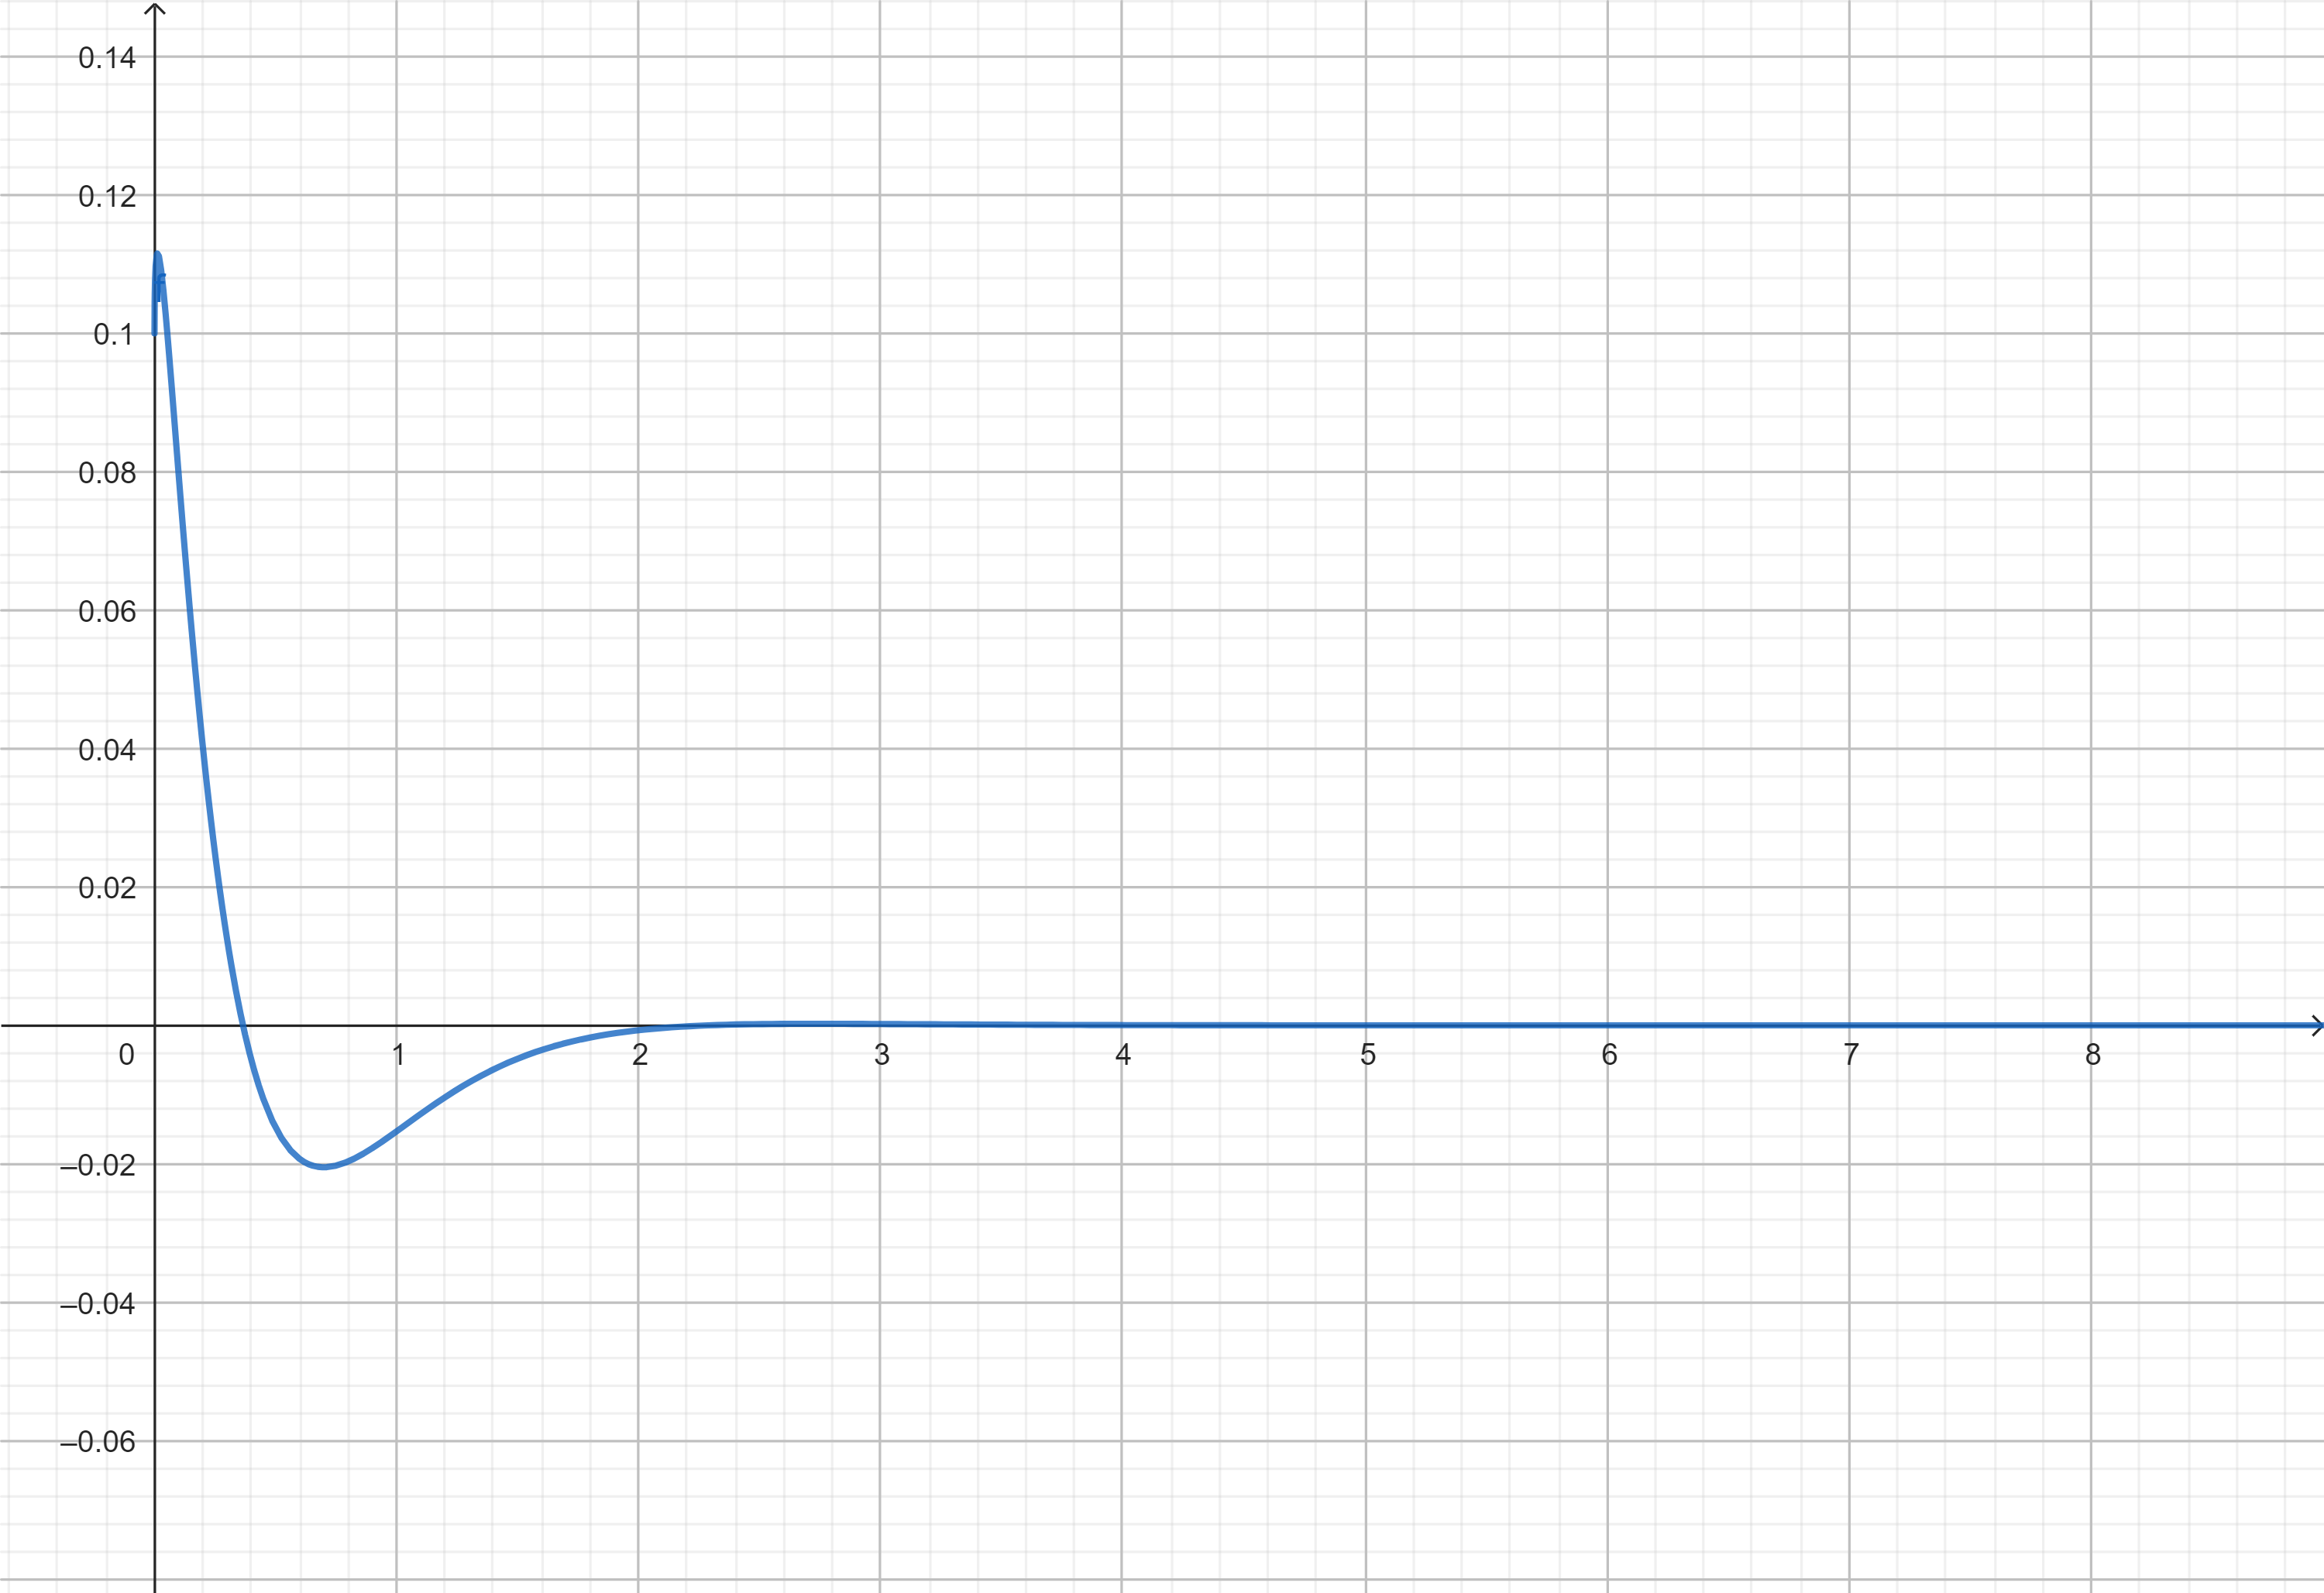
\includegraphics[width=0.8\textwidth]{imagen-ejercicio1.png}
        \caption{Gráfica de la solución $y(x) = e^{2x} - 2x e^{2x}$ generada con GeoGebra}
        \label{fig:ej1}
    \end{figure}
    
    \item \textbf{Ejercicio 2}: Encuentre la solución general de $y'' + 6y' + 13y = 0$.
    
    \textbf{Solución}: La ecuación característica es $r^2 + 6r + 13 = 0$, con raíces complejas $r = -3 \pm 2i$. La solución general es $y(x) = e^{-3x}(C_1 \cos(2x) + C_2 \sin(2x))$.
    
    Se empleó Python para simular numéricamente el comportamiento oscilatorio amortiguado de esta solución. Los resultados muestran oscilaciones que decaen exponencialmente, típicas de sistemas subamortiguados.
    
    \item \textbf{Ejercicio 3}: Resuelva el problema de valor inicial $2y'' + 4y' - 6y = 0$ con $y(0) = 2$, $y'(0) = 1$.
    
    \textbf{Solución}: La ecuación característica es $2r^2 + 4r - 6 = 0$, con raíces $r = 1$ y $r = -3$. La solución general es $y(x) = C_1 e^{x} + C_2 e^{-3x}$. Aplicando condiciones iniciales: $C_1 + C_2 = 2$ y $C_1 - 3C_2 = 1$, resolviendo obtenemos $C_1 = 1.75$, $C_2 = 0.25$. La solución particular es $y(x) = 1.75e^{x} + 0.25e^{-3x}$.
    
    \begin{figure}[h]
        \centering
        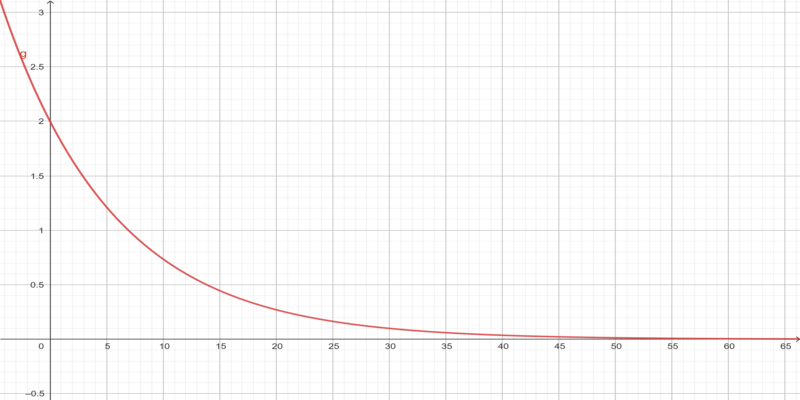
\includegraphics[width=0.8\textwidth]{imagen-ejercicio3.png}
        \caption{Diagrama de fase para el sistema asociado a $2y'' + 4y' - 6y = 0$ generado con GeoGebra}
        \label{fig:ej3}
    \end{figure}
    
    \item \textbf{Ejercicio 4}: Determine la solución general de $y^{(4)} - 16y = 0$.
    
    \textbf{Solución}: La ecuación característica es $r^4 - 16 = 0$, que factoriza como $(r^2 - 4)(r^2 + 4) = (r-2)(r+2)(r^2+4) = 0$. Las raíces son $r = 2$, $r = -2$, $r = 2i$, $r = -2i$. La solución general es:
    $$y(x) = C_1 e^{2x} + C_2 e^{-2x} + C_3 \cos(2x) + C_4 \sin(2x)$$
    
    \item \textbf{Ejercicio 5}: Un circuito RLC serie tiene $L = 1$ H, $R = 10$ Ω, $C = 0.04$ F. Encuentre la ecuación diferencial para la carga $q(t)$ y resuélvala si $q(0) = 5$, $q'(0) = 0$.
    
    \textbf{Solución}: La ecuación diferencial es:
    $$1 \cdot q'' + 10 q' + \frac{1}{0.04} q = 0 \Rightarrow q'' + 10q' + 25q = 0$$
    
    La ecuación característica es $r^2 + 10r + 25 = 0$, con raíz doble $r = -5$. La solución general es $q(t) = C_1 e^{-5t} + C_2 t e^{-5t}$. Aplicando condiciones iniciales: $C_1 = 5$, $C_2 = 25$. La solución particular es $q(t) = 5e^{-5t} + 25t e^{-5t}$.
    
    Se utilizó Python para simular numéricamente la respuesta del circuito, mostrando cómo la carga decae críticamente amortiguada hacia cero.
    
    \begin{figure}[h]
        \centering
        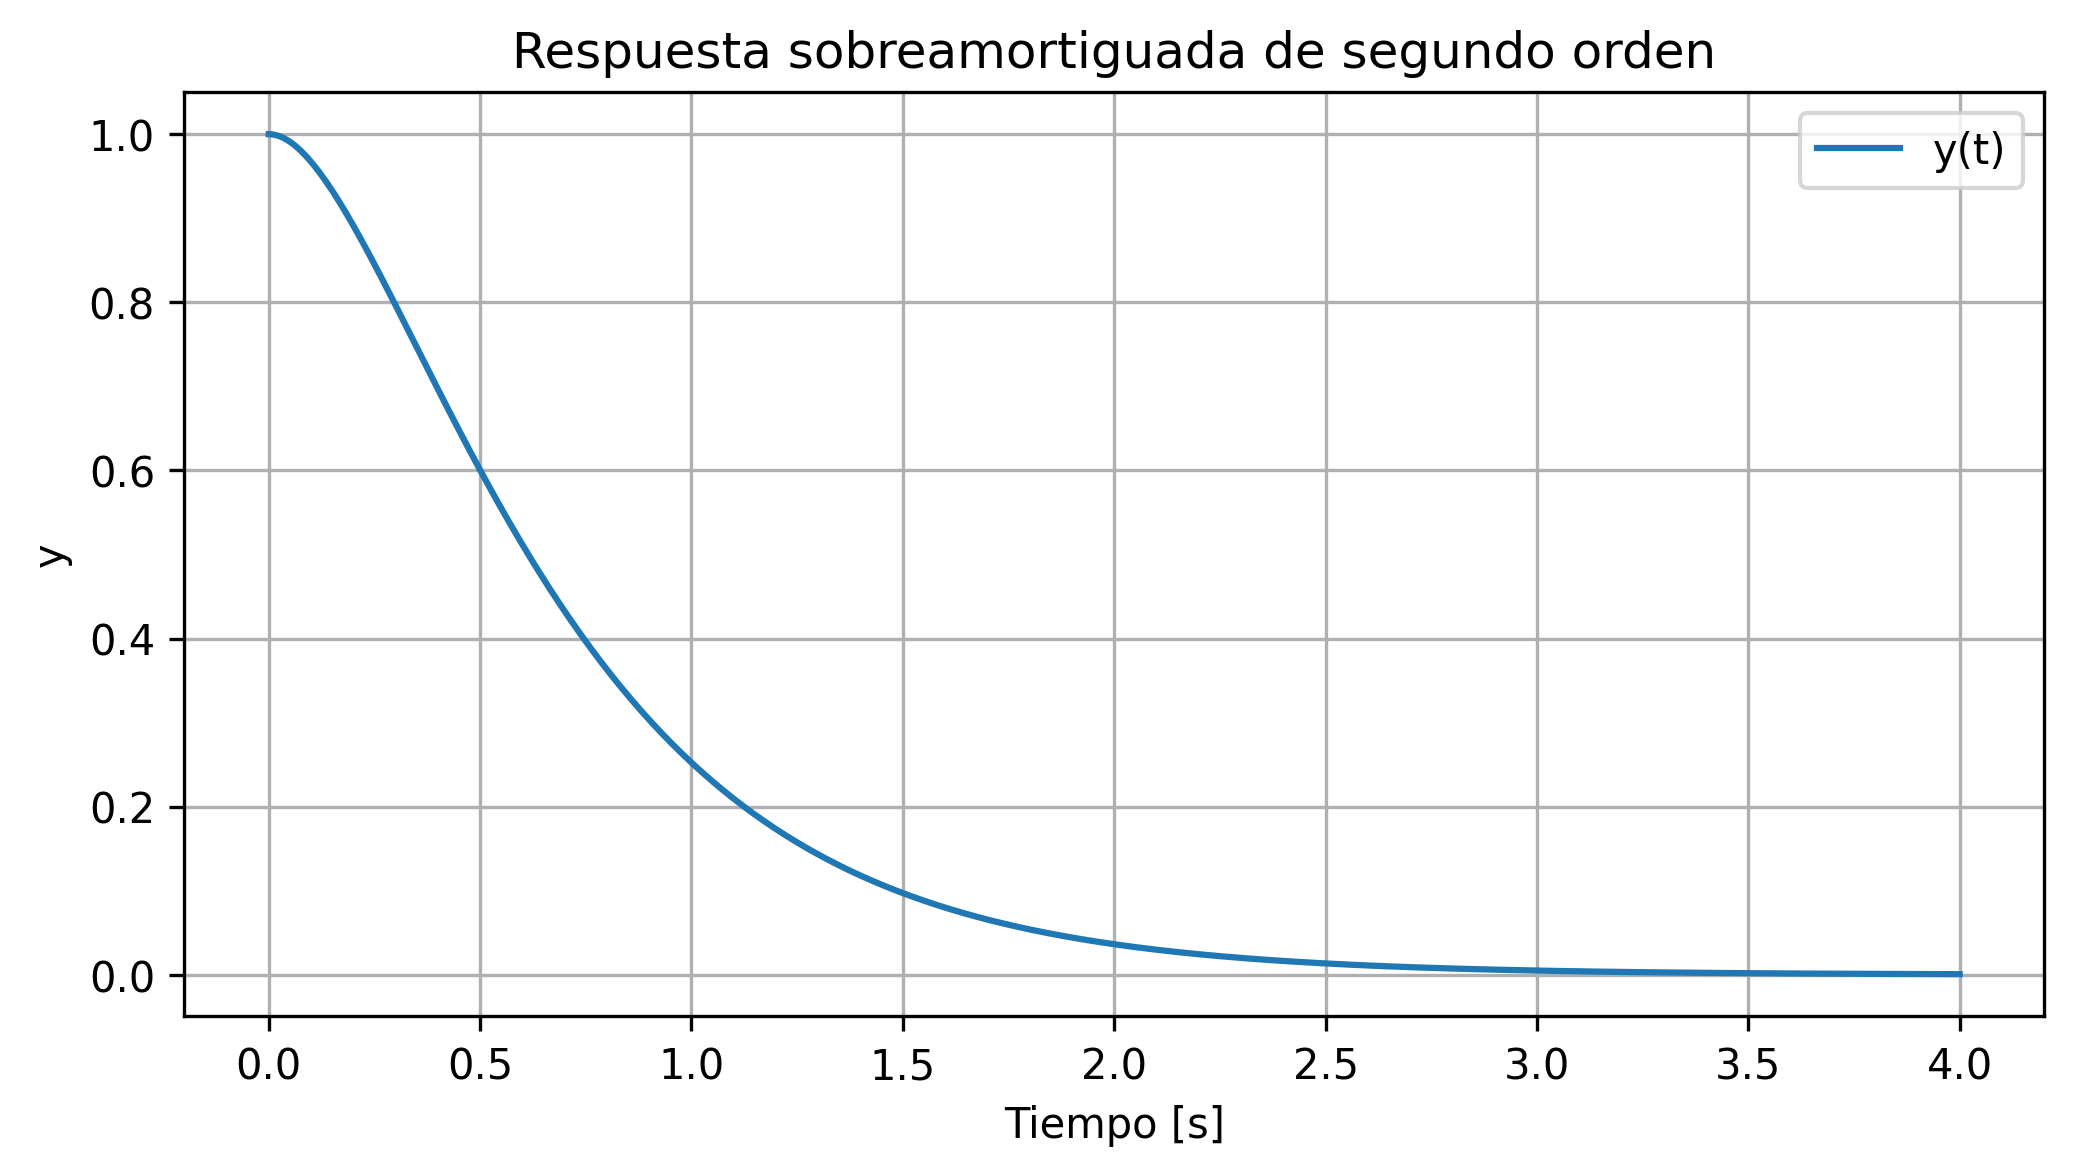
\includegraphics[width=0.8\textwidth]{imagen-ejercicio5.png}
        \caption{Respuesta del circuito RLC críticamente amortiguado generada con Python y matplotlib}
        \label{fig:ej5}
    \end{figure}
\end{enumerate}

% ============================
% PÁGINA 10: CONCLUSIÓN
% ============================
\section{Conclusión}

Las ecuaciones diferenciales homogéneas con coeficientes lineales constituyen una herramienta matemática esencial en el arsenal del ingeniero de sistemas. Su estudio proporciona las bases teóricas necesarias para comprender y modelar una amplia gama de sistemas dinámicos, desde circuitos eléctricos hasta sistemas de control automático.

El método de la ecuación característica para coeficientes constantes ofrece un procedimiento sistemático y eficaz para resolver estas ecuaciones, mientras que el principio de superposición garantiza la completitud de las soluciones encontradas. Las aplicaciones prácticas en ingeniería, particularmente en el análisis de circuitos RLC y sistemas masa-resorte-amortiguador, demuestran la relevancia de estos conceptos en contextos reales.

La incorporación de herramientas computacionales como GeoGebra para visualización gráfica y Python para simulación numérica enriquece sustancialmente el análisis, permitiendo una comprensión más intuitiva del comportamiento de las soluciones. No obstante, es fundamental mantener una sólida comprensión de los principios teóricos subyacentes para interpretar correctamente los resultados obtenidos mediante estas herramientas.

Como extensiones futuras de este trabajo, se sugiere explorar ecuaciones con coeficientes variables, sistemas de ecuaciones diferenciales acoplados y aplicaciones avanzadas en teoría de control moderno, donde estos conceptos encuentran aplicaciones adicionales en el diseño de controladores robustos y sistemas adaptativos.

% ============================
% REFERENCIAS BIBLIOGRÁFICAS
% ============================
\bibliographystyle{apacite}
\bibliography{referencias}

\begin{thebibliography}{10}

\bibitem{baraniuk}
Baraniuk, R. G. et al. (2020). \textit{Ecuaciones diferenciales de coeficiente constante lineal}. LibreTexts Español. Recuperado de https://espanol.libretexts.org/Ingenier\%C3\%ADa/Senales\_y\_Sistemas/

\bibitem{openstax}
OpenStax. (2021). \textit{Cálculo volumen 3: Ecuaciones lineales de segundo orden}. OpenStax. Recuperado de https://openstax.org/books/c\%C3\%A1lculo-volumen-3/pages/7-1-ecuaciones-lineales-de-segundo-orden

\bibitem{normasapa}
Sánchez, C. (2019). \textit{Normas APA – 7ma (séptima) edición}. Normas APA. Recuperado de https://normas-apa.org/

\bibitem{overleaf}
Overleaf. (2023). \textit{Inserting Images}. Overleaf Documentation. Recuperado de https://es.overleaf.com/learn/latex/Inserting\_Images

\bibitem{spie}
SPIE. (2008). \textit{SPIE LaTeX manuscript templates and writing guidelines}. Universidad del País Vasco. Recuperado de https://www.ehu.eus/ccwintco/index.php/SPIE\_LaTEX\_manuscript\_templates\_and\_writing\_guidelines

\end{thebibliography}

\end{document}